% ============================================================
% Rapport écrit ESP — DeadlockHelper
% Anthony Boily | 420-VC2-LP | 03 juin 2026
% Compiler : pdflatex rapport_final.tex (depuis docs/latex/)
% ============================================================
\documentclass[12pt,a4paper]{article}

\usepackage[utf8]{inputenc}
\usepackage[T1]{fontenc}
\usepackage[english]{babel} % TEMP: changer en [french] apres: sudo pacman -S texlive-langfrench
\usepackage[top=2.5cm, bottom=2.5cm, left=2.5cm, right=2.5cm]{geometry}
\usepackage{graphicx}
\usepackage[colorlinks=true,
            linkcolor=blue!60!black,
            urlcolor=blue!60!black]{hyperref}
\usepackage{xcolor}
\usepackage{listings}
\usepackage{tikz}
\usepackage{tikz-qtree}
\usepackage{fancyhdr}
\usepackage{float}
\usepackage{booktabs}
\usepackage{array}
\usepackage{parskip}
\usepackage{microtype}
\usepackage{enumitem}

\usetikzlibrary{arrows.meta, positioning, shapes.geometric, backgrounds}

% ── Images : chercher dans docs/ et src/assets/Images/ depuis docs/latex/
% NOTE : les images doivent être accessibles aux chemins relatifs indiqués.
\graphicspath{{../}{../../src/assets/Images/}}

% ── Couleurs personnalisées ───────────────────────────────────────────────────
\definecolor{codebg}{RGB}{248,248,250}
\definecolor{codeframe}{RGB}{210,210,215}
\definecolor{codekw}{RGB}{0,0,180}
\definecolor{codestr}{RGB}{163,21,21}
\definecolor{codecomment}{RGB}{106,153,85}
\definecolor{codenumber}{RGB}{150,150,150}
\definecolor{rarity-epic}{RGB}{160,32,240}
\definecolor{rarity-rare}{RGB}{0,112,221}
\definecolor{rarity-common}{RGB}{100,100,100}
\definecolor{rarity-infamous}{RGB}{180,0,0}
\definecolor{rarity-uncommon}{RGB}{38,169,92}

% ── Configuration listings ───────────────────────────────────────────────────
\lstdefinelanguage{TypeScript}{
  language=Java,
  morekeywords={type, interface, readonly, abstract, implements, declare,
                namespace, module, enum, keyof, typeof, as, infer, is,
                string, number, boolean, void, null, undefined, any,
                const, let, var, function, return, import, export, from,
                async, await, extends, new, class, public, private, protected},
  sensitive=true,
  morecomment=[l]{//},
  morecomment=[s]{/*}{*/},
  morestring=[b]',
  morestring=[b]",
  morestring=[b]`,
}

\lstset{
  basicstyle=\ttfamily\footnotesize,
  keywordstyle=\color{codekw}\bfseries,
  stringstyle=\color{codestr},
  commentstyle=\color{codecomment}\itshape,
  numberstyle=\tiny\color{codenumber},
  numbers=left,
  numbersep=8pt,
  backgroundcolor=\color{codebg},
  frame=single,
  rulecolor=\color{codeframe},
  breaklines=true,
  breakatwhitespace=false,
  tabsize=2,
  showstringspaces=false,
  captionpos=b,
  xleftmargin=15pt,
  framexleftmargin=15pt,
}

% ── En-têtes et pieds de page ─────────────────────────────────────────────────
\pagestyle{fancy}
\fancyhf{}
\fancyhead[L]{\small\textit{DeadlockHelper --- Rapport écrit ESP}}
\fancyhead[R]{\small Anthony Boily}
\fancyfoot[C]{\thepage}
\renewcommand{\headrulewidth}{0.4pt}
\setlength{\headheight}{15pt}

% ── Métadonnées PDF ───────────────────────────────────────────────────────────
\hypersetup{
  pdftitle={Rapport écrit ESP --- DeadlockHelper},
  pdfauthor={Anthony Boily},
  pdfsubject={Projet professionnel 2 --- 420-VC2-LP},
}

% =============================================================================
\begin{document}
% =============================================================================

% ─────────────────────────────────────────────────────────────────────────────
% PAGE DE PRÉSENTATION
% ─────────────────────────────────────────────────────────────────────────────
\begin{titlepage}
  \centering
  \vspace*{2.5cm}

  {\LARGE\bfseries ANTHONY BOILY\par}
  \vspace{0.6cm}
  {\large Projet professionnel 2\par}
  {\large 420-VC2-LP\par}

  \vfill

  {\Huge\bfseries Rapport écrit ESP\par}
  \vspace{2cm}

  {\large\bfseries Travail présenté à~:\par}
  \vspace{0.4cm}
  {\large\bfseries Michel Forget et Nicolas Demers\par}

  \vfill

  {\large Techniques de l'informatique\par}
  {\large Cégep de La Pocatière\par}
  \vspace{0.8cm}
  {\large 03 juin 2026\par}
\end{titlepage}

% ─────────────────────────────────────────────────────────────────────────────
% TABLE DES MATIÈRES
% ─────────────────────────────────────────────────────────────────────────────
\newpage
\tableofcontents

% ─────────────────────────────────────────────────────────────────────────────
% TABLE DES FIGURES
% ─────────────────────────────────────────────────────────────────────────────
\newpage
\listoffigures

% ─────────────────────────────────────────────────────────────────────────────
% CORPS DU RAPPORT
% ─────────────────────────────────────────────────────────────────────────────
\newpage

% ═══════════════════════════════════════════════════════════════════════════
\section{Identification du projet}
% ═══════════════════════════════════════════════════════════════════════════

Mon projet consiste à développer une application compagnon et d'assistance
en temps réel, pour optimiser l'expérience des joueurs et analyser leurs
statistiques sur le jeu vidéo \textit{Deadlock}, un jeu de tir tactique
multijoueur en ligne développé par Valve.

% ═══════════════════════════════════════════════════════════════════════════
\section{Description sommaire du projet}
% ═══════════════════════════════════════════════════════════════════════════

\textit{DeadlockHelper} est une application de bureau multiplateforme
(Windows et Linux) conçue pour fonctionner en arrière-plan pendant que
l'utilisateur joue à \textit{Deadlock}. Elle est distribuée gratuitement
à l'adresse \url{https://diredoch.github.io/DeadlockHelper/} sous forme
d'un fichier \texttt{.AppImage} pour Linux et d'un installateur \texttt{.exe}
pour Windows.

L'application est structurée autour de plusieurs onglets thématiques
adaptés au cycle de vie du joueur. \textbf{Hors-partie}, elle sert de
centre de connaissances~: bibliothèque de héros, explorateur de
\textit{builds} d'objets recommandés par la communauté, et onglet
\textit{Profil} affichant l'historique de matchs assorti d'un
système d'Awards calculés sur les performances réelles de l'utilisateur.
\textbf{En partie}, un overlay transparent se superpose au jeu pour
afficher des timers (Mid Boss, Urne) et des suggestions d'objets contre
la composition adverse. \textbf{Post-partie}, le \textit{Live Dashboard}
regroupe les tuiles statistiques de tous les joueurs d'un match récent
sur une grille de 6~$\times$~2.

Un widget Spotify intégré permet de contrôler la musique (lecture, pause,
piste suivante, rewind) sans quitter l'application. La synchronisation
avec le compte Steam de l'utilisateur est requise pour récupérer son
profil et ses données de matchs via l'API communautaire
\textit{Deadlock-API.com}.

\begin{figure}[htbp]
  \centering
  % NOTE : image dans docs/ReadmeHeroes.png (chemin relatif depuis docs/latex/)
  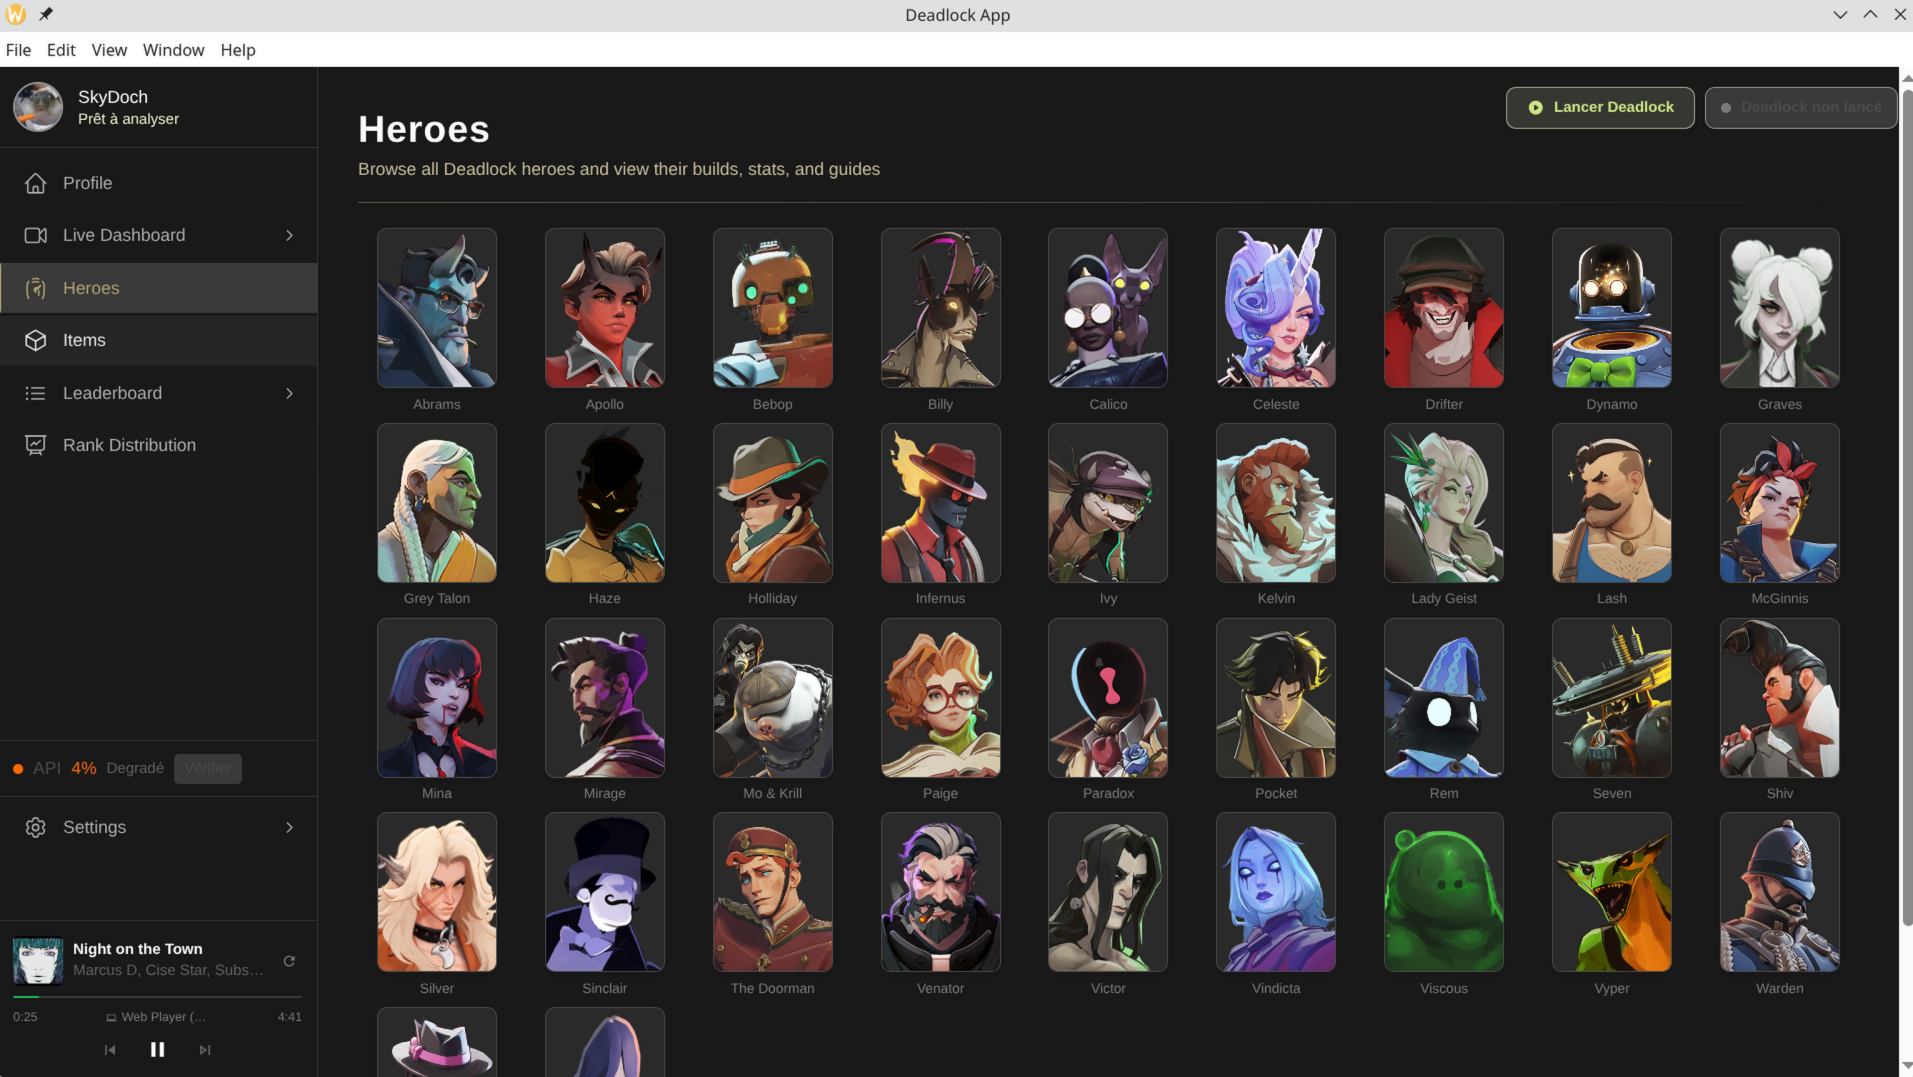
\includegraphics[width=0.88\textwidth]{ReadmeHeroes.png}
  \caption{Bibliothèque de héros --- vue principale de l'application}
  \label{fig:heroes}
\end{figure}

% ═══════════════════════════════════════════════════════════════════════════
\section{Identification des domaines de l'informatique concernés}
% ═══════════════════════════════════════════════════════════════════════════

Ce projet mobilise la majorité des domaines enseignés dans le cadre du DEC
en Techniques de l'informatique. Le tableau suivant présente chaque domaine
avec le cours associé et son application concrète dans le projet~:

\vspace{0.5em}
\begin{center}
\begin{tabular}{>{\bfseries}p{4.2cm} p{2.5cm} p{6.5cm}}
\toprule
Domaine & Cours & Application dans le projet \\
\midrule
Développement web & 420-VBA-LP & Interface Electron, TypeScript, HTML/CSS \\
Prog. web dynamique & 420-V88-LP & Vite, routing, composants UI asynchrones \\
Prog. orientée objet & 420-V83-LP & Interfaces TypeScript, entités Player/Match \\
Systèmes d'exploitation & 420-V89-LP & Processus Linux/Windows, fichiers config \\
Sécurité et automatisation & 420-VB6-LP & Scripts CI/CD, packaging .AppImage/.exe \\
Algorithmique & 420-V80-LP & Calculs métriques, filtrage JSON volumineux \\
Programmation avancée & 420-VA9-LP & Python 3.12, EasyOCR, traitement de données \\
Base de données & 420-V91-LP & electron-store, cache local, TTL 7~jours \\
Développement de jeux & 420-VC3-LP & Contexte Deadlock, overlay in-game \\
Gestion de projet & 420-VB9-LP & Kanban, GitHub, planification Agile \\
Mathématiques appliquées & 201-V03-LP & Pondération statistique des Awards \\
Algèbre et statistiques & 201-V04-LP & Seuils de performance, percentiles \\
\bottomrule
\end{tabular}
\end{center}

% ═══════════════════════════════════════════════════════════════════════════
\section{Réalisation du projet}
% ═══════════════════════════════════════════════════════════════════════════

\subsection{Application de bureau téléchargeable}

L'application est distribuée via GitHub Pages. La compilation est
automatisée par GitHub Actions~: à chaque version taguée, le pipeline
produit un \texttt{.AppImage} autosuffisant pour Linux et un installateur
\texttt{.exe} pour Windows. L'utilisateur n'a aucun prérequis à installer
manuellement.

\subsection{Widget Spotify intégré}

Le widget Spotify permet de contrôler la musique directement depuis
l'application~: lecture, pause, piste suivante et piste précédente.
L'authentification repose sur le flux
\textit{Authorization Code with PKCE} de l'API Spotify Web~: aucun secret
client n'est stocké dans le code compilé. Les jetons d'accès (valides
1~heure) et de rafraîchissement sont persistés localement.

\begin{figure}[htbp]
  \centering
  % NOTE : image dans docs/SpotifyWidget.png
  
\includegraphics[width=0.52\textwidth]{SpotifyWidget.png}
  \caption{Widget Spotify --- contrôles de lecture et pochette d'album}
  \label{fig:spotify}
\end{figure}

\subsection{Synchronisation Steam et données Deadlock}

L'authentification Steam utilise le protocole OpenID, qui redirige
l'utilisateur vers la page officielle de Valve sans jamais exposer son
mot de passe à l'application. Une fois connecté, l'application récupère
le \texttt{SteamID64} et interroge \textit{Deadlock-API.com} pour
l'historique de matchs, les statistiques par héros et le rang.

\subsection{Système d'Awards}

Le système d'Awards analyse l'historique de matchs et attribue des
médailles de performance. Il regroupe 48~awards en 5~raretés~:
\textit{Common}, \textit{Uncommon}, \textit{Rare}, \textit{Epic} et
\textit{Infamous}. Chaque award est calculé à partir du champ
\texttt{stats[]} de l'API (données de fin de match)~: dégâts par minute,
âmes par minute, taux de participation aux éliminations, précision de tir,
etc.

\begin{figure}[htbp]
  \centering
  % NOTE : image dans docs/ReadmeProfilAwards.png
  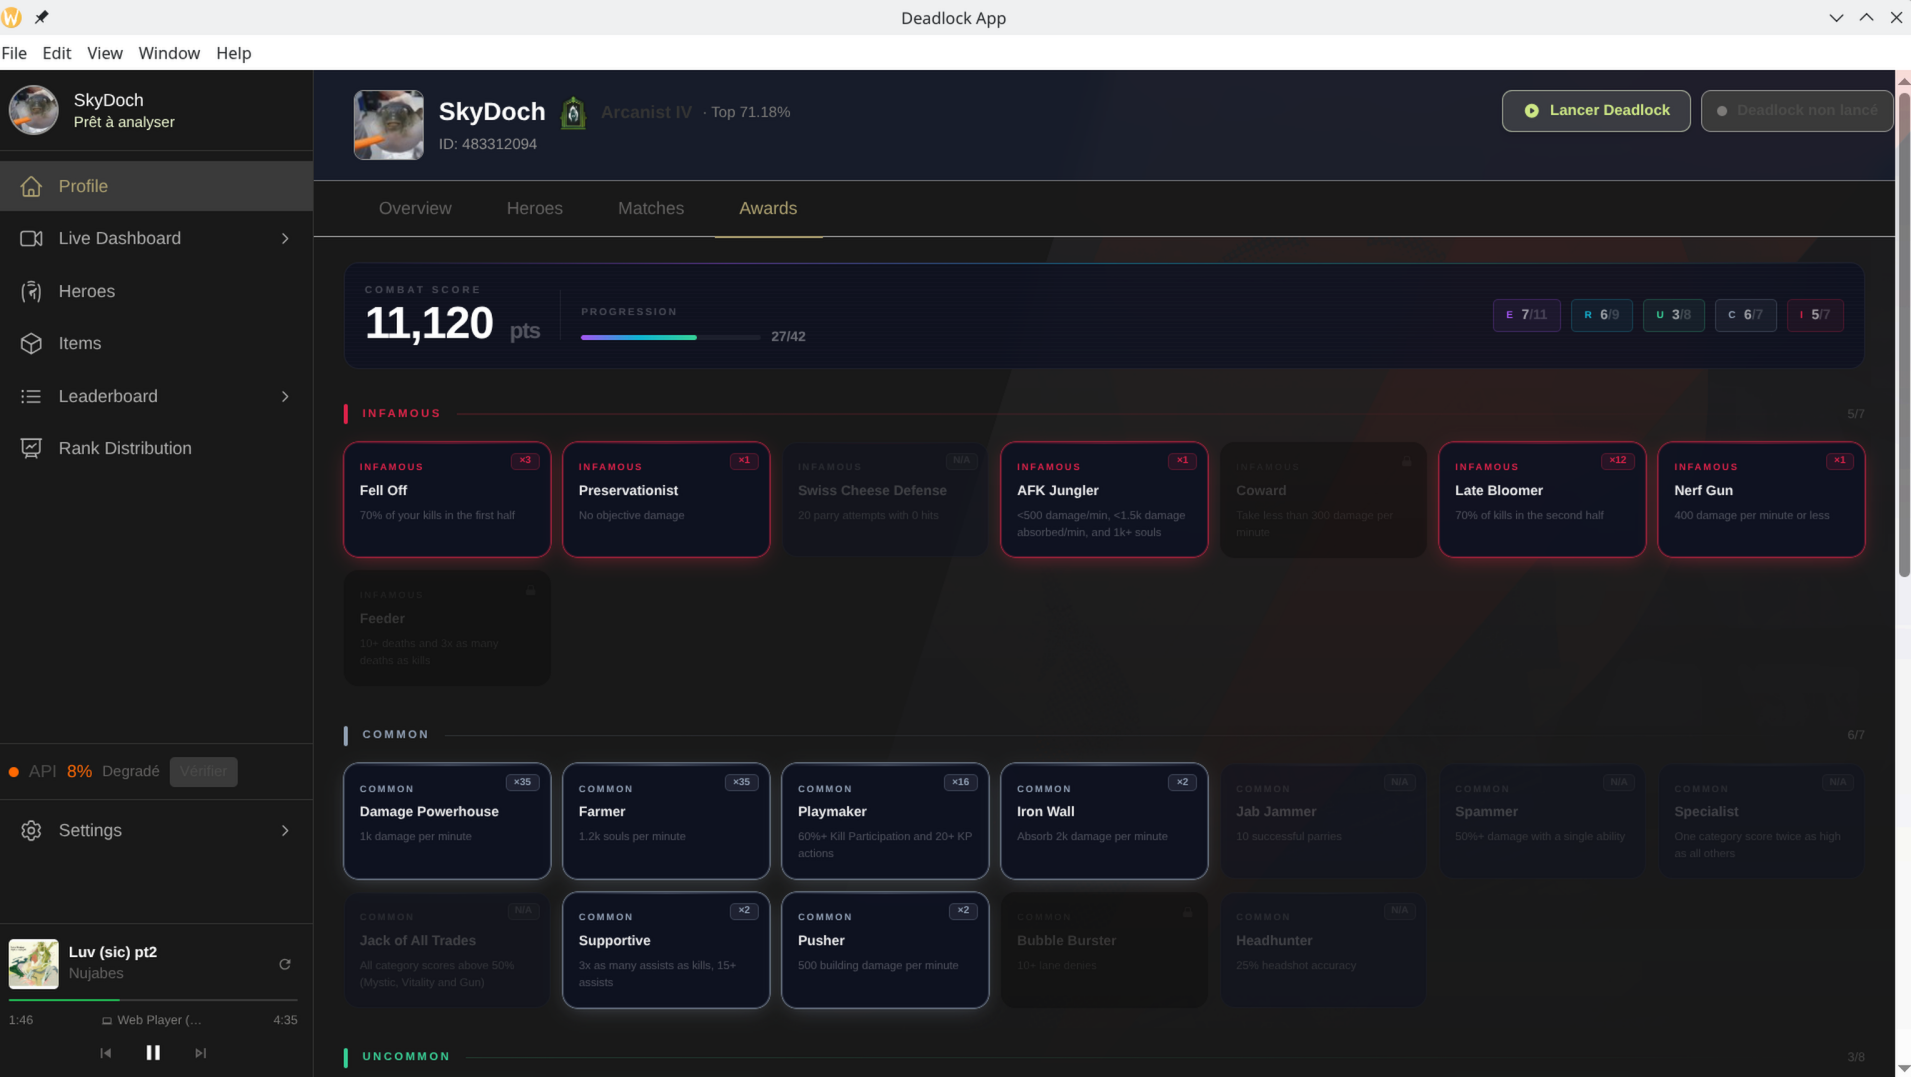
\includegraphics[width=0.88\textwidth]{ReadmeProfilAwards.png}
  \caption{Page Profil --- système d'Awards avec raretés et statistiques}
  \label{fig:awards-page}
\end{figure}

\subsection{Game Overlay transparent}

L'overlay in-game est une seconde fenêtre Electron
(\texttt{BrowserWindow}) configurée avec \texttt{frame:~false},
\texttt{transparent:~true} et \texttt{alwaysOnTop:~true}. Elle se
superpose au jeu sans perturber son déroulement, avec quatre composants~:
un timer Mid Boss (déclenché manuellement), un timer d'Urne (déterministe,
calculé depuis l'horloge de partie), des suggestions d'objets contre la
composition ennemie, et un indicateur \texttt{Souls/min} (placeholder).

\begin{figure}[htbp]
  \centering
  % NOTE : image dans src/assets/Images/GameOverlayExemple.png
  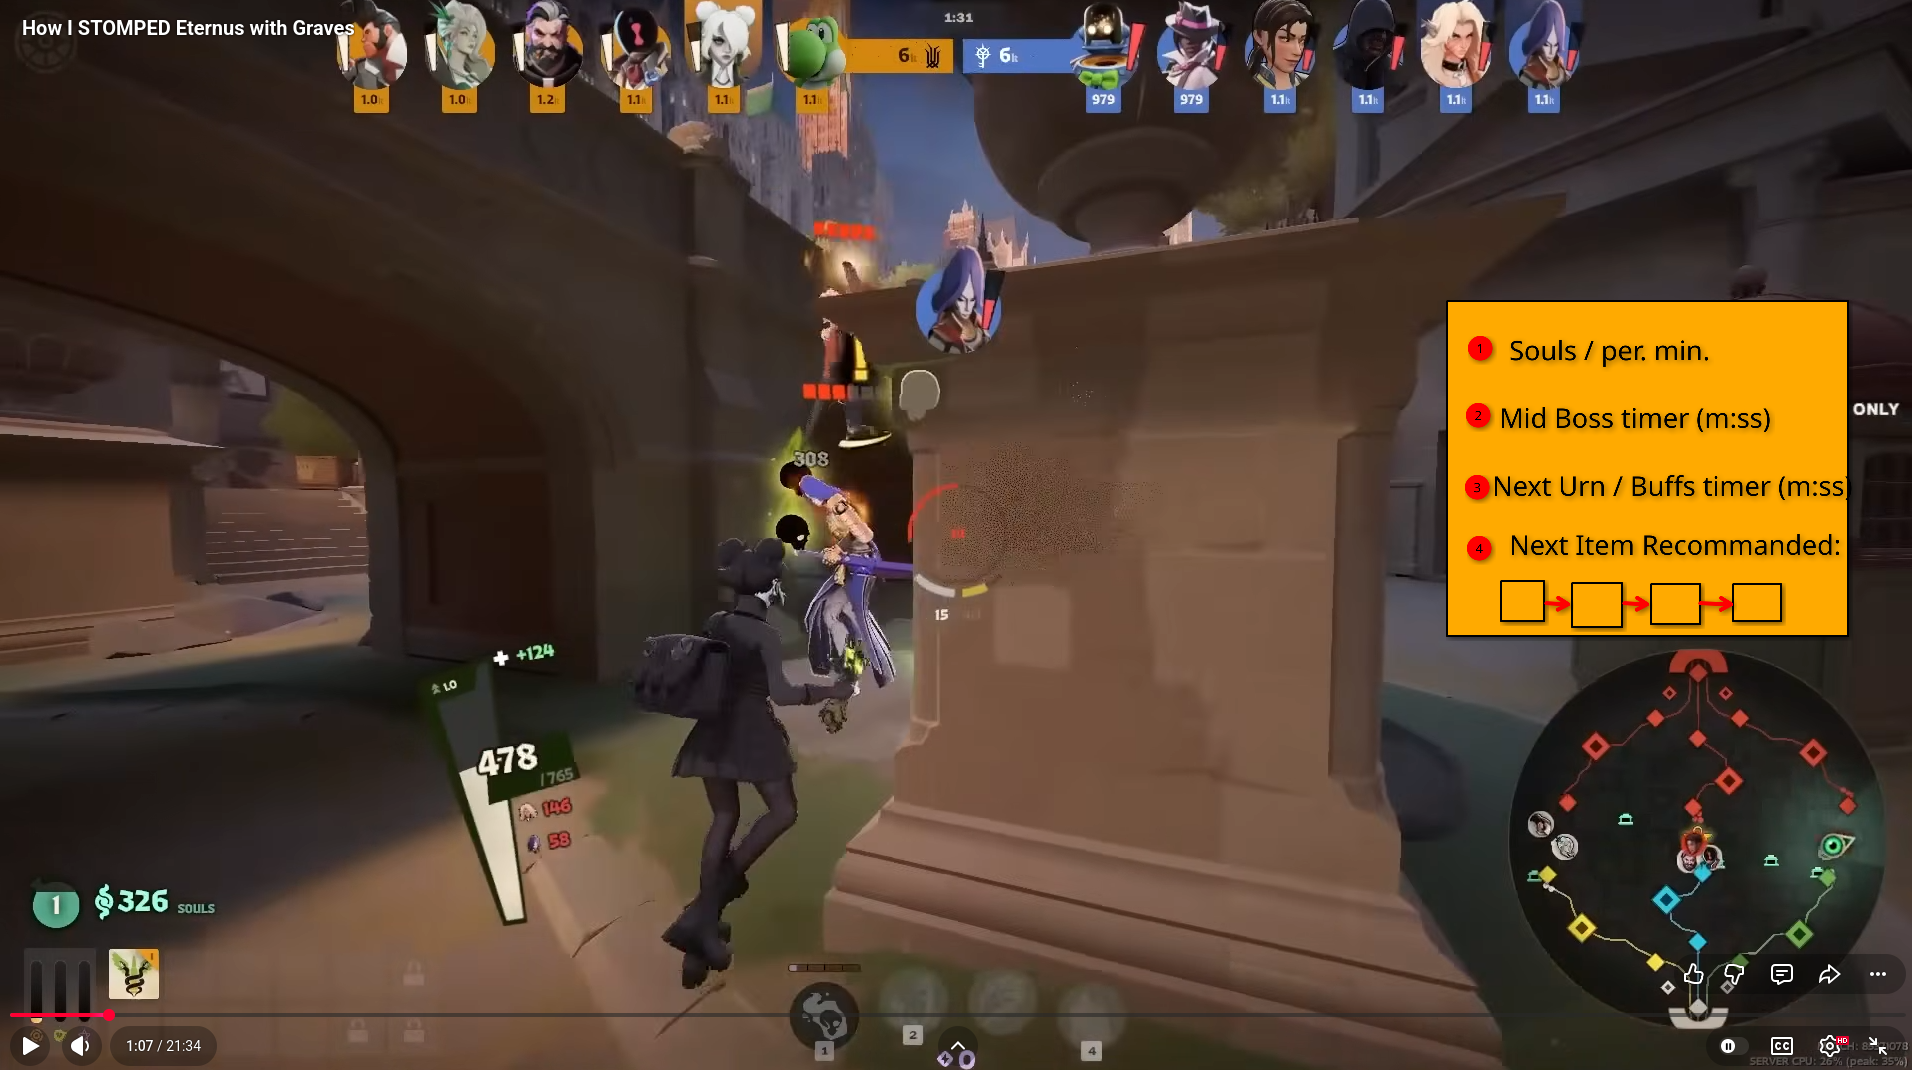
\includegraphics[width=0.88\textwidth]{GameOverlayExemple.png}
  \caption{Game Overlay --- superposition transparente par-dessus le jeu}
  \label{fig:overlay}
\end{figure}

\subsection{Live Dashboard}

Le Live Dashboard affiche les 12~joueurs d'un match sous forme de
grille. Il récupère le roster via le \textit{bulk metadata endpoint}
de l'API (\texttt{GET /v1/matches/metadata?match\_ids=\{id\}}), qui
tolère 10~requêtes par minute sans dépendance Steam, contrairement au
endpoint unitaire limité à 3~requêtes par heure.

\begin{figure}[htbp]
  \centering
  % NOTE : image dans docs/ReadmeLiveDashboard.png
  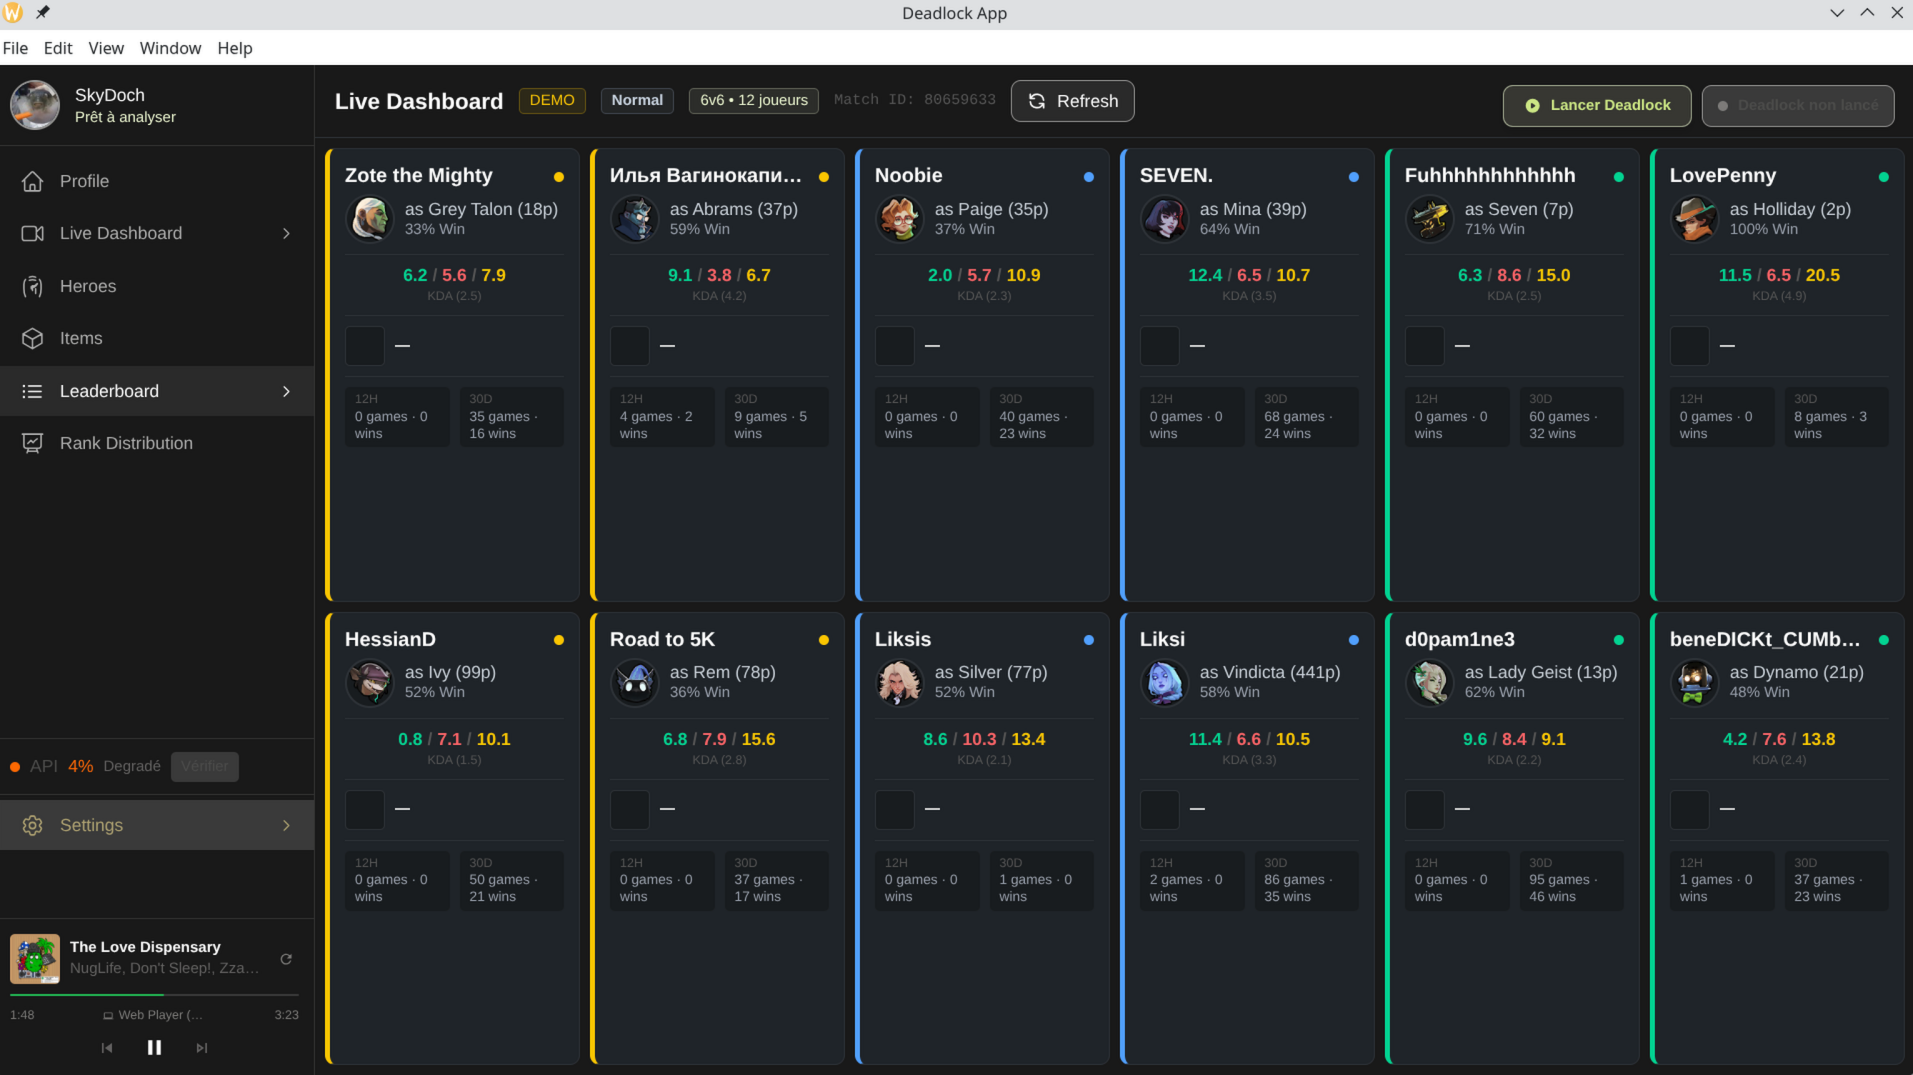
\includegraphics[width=0.88\textwidth]{ReadmeLiveDashboard.png}
  \caption{Live Dashboard --- grille des 12~joueurs avec statistiques}
  \label{fig:dashboard}
\end{figure}

% ═══════════════════════════════════════════════════════════════════════════
\section{Comment le projet a été réalisé}
% ═══════════════════════════════════════════════════════════════════════════

\subsection{Méthodologie et outils de planification}

Le projet a été planifié et suivi avec \textbf{Microsoft Planner} selon
un tableau Kanban. Chaque fonctionnalité a été découpée en tâches
étiquetées selon leur priorité~: \textit{MVP} (ce qui doit absolument
figurer dans la démonstration finale) ou \textit{Backlog} (améliorations
à venir). Cette distinction a permis de livrer un produit fonctionnel dans
les délais tout en gardant une vision claire des fonctionnalités futures.

En parallèle, un vault \textbf{Obsidian} a servi de base de connaissances
personnelle, avec notamment un diagramme \textit{Excalidraw} dessiné sur
1 à 2~semaines avant le début du code pour visualiser l'architecture
globale, la navigation entre onglets et les flux de données entre les API.
Cette étape s'est révélée cruciale pour anticiper les dépendances et les
risques techniques.

Un \textbf{PRD} (\textit{Product Requirement Document}) a été rédigé pour
recenser toutes les sources externes nécessaires~: clés API à obtenir,
portails développeur à consulter, contraintes d'authentification à
respecter.

\subsection{Étapes de réalisation}

\begin{enumerate}[leftmargin=*, label=\textbf{\arabic*.}]
  \item \textbf{Planification Kanban~:} découpage des fonctionnalités en
    tâches individuelles, étiquetage MVP~vs.~Backlog dans Microsoft
    Planner.
  \item \textbf{Prototypage visuel~:} modélisation de l'architecture et
    des écrans dans Excalidraw (vault Obsidian) pour valider la vision
    globale avant de coder.
  \item \textbf{PRD~:} recensement exhaustif des API, portails
    développeur, clés et contraintes d'accès.
  \item \textbf{Validation des technologies risquées en premier~:}
    authentification Steam (OpenID) et Spotify (OAuth PKCE), heartbeat
    de disponibilité de l'API Deadlock --- prouver que le \textit{stack}
    fonctionne avant d'investir dans l'interface.
  \item \textbf{Construction de l'interface~:} charte de couleurs
    définie en CSS, arborescence de fichiers structurée, navigation
    fonctionnelle, pages marquées «~En cours de développement~» comme
    placeholders.
  \item \textbf{Développement itératif~:} implémentation des
    fonctionnalités par ordre décroissant de risque et de complexité,
    avec commits réguliers et documentation des décisions
    architecturales (ADR).
\end{enumerate}

\subsection{Environnement de développement}

Le développement s'est déroulé sur deux systèmes~: Windows avec l'IDE
\textit{Cursor} (version de VS~Code enrichie de fonctionnalités d'IA
générative) et Linux CachyOS avec \textit{Code~OSS} (version open-source
de VS~Code). \textit{NeoVIM} a été expérimenté comme éditeur secondaire.
Git et GitHub ont servi pour la gestion de version et le CI/CD.

% ═══════════════════════════════════════════════════════════════════════════
\section{Technologies choisies}
% ═══════════════════════════════════════════════════════════════════════════

\subsection{Architecture Electron et communication IPC}

Le cœur de l'application repose sur \textbf{Electron~40.0.0} couplé à
\textbf{Vite} et \textbf{TypeScript}. Electron permet de créer des
applications de bureau avec les technologies web tout en donnant accès aux
API système (fichiers, processus, réseau). Son architecture est
\textbf{multi-processus}~: un processus principal (\texttt{main.ts}) gère
les fenêtres et les appels système, un ou plusieurs processus de rendu
constituent l'interface graphique. La communication entre les deux passe
par un canal sécurisé appelé \textbf{IPC}
(\textit{Inter-Process Communication}).

\begin{figure}[htbp]
  \centering
  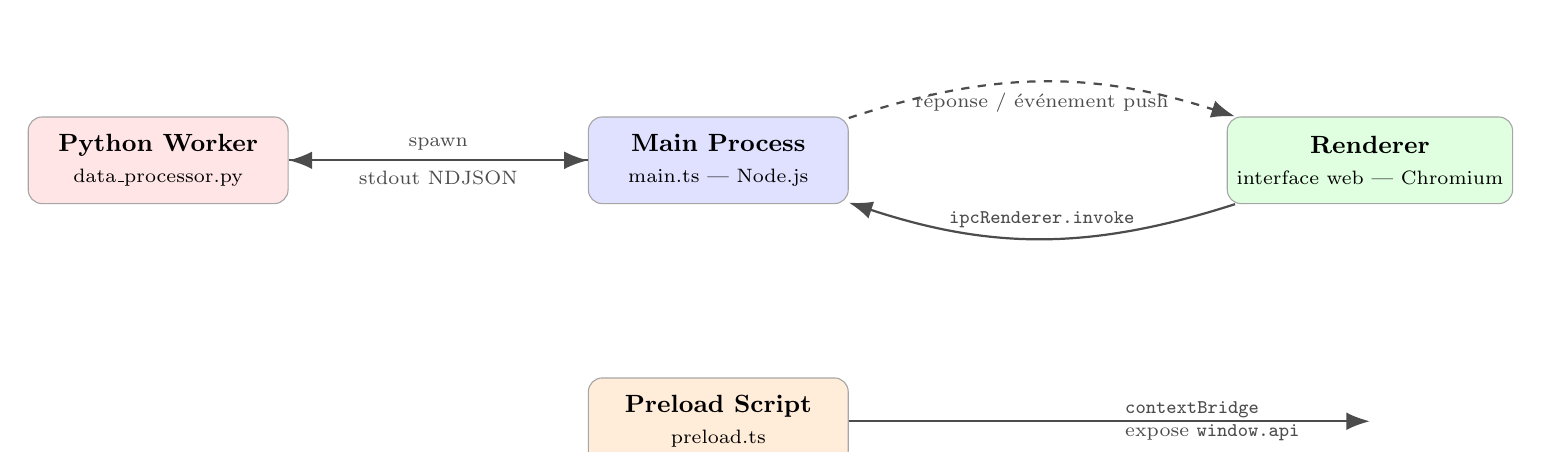
\begin{tikzpicture}[
    node distance=1.8cm,
    pbox/.style={rectangle, draw=gray!70, rounded corners=5pt,
                 minimum width=3.3cm, minimum height=1.1cm,
                 align=center, font=\small},
    arr/.style={-{Latex[length=3mm]}, thick, gray!60!black},
    darr/.style={-{Latex[length=3mm]}, thick, dashed, gray!60!black},
  ]
    \node[pbox, fill=blue!12]  (main)     {\textbf{Main Process}\\
                                            {\scriptsize main.ts --- Node.js}};
    \node[pbox, fill=orange!15, below=2.2cm of main] (preload)
                                           {\textbf{Preload Script}\\
                                            {\scriptsize preload.ts}};
    \node[pbox, fill=green!12, right=4.8cm of main] (renderer)
                                           {\textbf{Renderer}\\
                                            {\scriptsize interface web --- Chromium}};
    \node[pbox, fill=red!10, left=3.8cm of main] (python)
                                           {\textbf{Python Worker}\\
                                            {\scriptsize data\_processor.py}};

    % Main <-> Python
    \draw[arr]  (main)    -- node[above, font=\scriptsize]{spawn}         (python);
    \draw[darr] (python)  -- node[below, font=\scriptsize]{stdout NDJSON} (main);

    % Preload -> Renderer (contextBridge)
    \draw[arr]  (preload) -- node[right=2pt, font=\scriptsize, align=left]
                               {\texttt{contextBridge}\\expose \texttt{window.api}}
                               (renderer |- preload);

    % Renderer -> Main (invoke)
    \draw[arr, bend left=18]  (renderer) to
      node[above, font=\scriptsize]{\texttt{ipcRenderer.invoke}} (main);

    % Main -> Renderer (response / event push)
    \draw[darr, bend left=18] (main) to
      node[below, font=\scriptsize]{réponse / événement push} (renderer);
  \end{tikzpicture}
  \caption{Architecture multi-processus Electron --- flux IPC et Context Bridge}
  \label{fig:ipc-arch}
\end{figure}

Le \textbf{Context Bridge} est le pont de sécurité entre le preload et
le renderer. Il expose uniquement les fonctions autorisées via
\texttt{window.api}, sans jamais donner au renderer un accès direct à
Node.js.

\begin{lstlisting}[language=TypeScript,
  caption={Extrait de preload.ts --- exposition sécurisée via contextBridge}]
contextBridge.exposeInMainWorld('api', {
  // Requete generique vers le processus principal
  request: (endpoint: string, options?: { method?: string; body?: any }) =>
    ipcRenderer.invoke('api:request', { endpoint, ...options }),

  // Authentification Steam (OpenID)
  steamStartAuth: () =>
    ipcRenderer.invoke('steam:startAuth'),

  // Disponibilite de l'API Deadlock (heartbeat)
  getApiAvailability: () =>
    ipcRenderer.invoke('api:get-availability'),

  // Push du main vers renderer : alertes de sante de l'API
  onHealthStatusChange: (callback: (availability: number) => void) => {
    ipcRenderer.on('api:health-alert', (_event, availability: number) => {
      callback(availability);
    });
  },
});
\end{lstlisting}

\bigskip

La figure~\ref{fig:class_diagram} représente les principales entités manipulées par l'application sous forme de diagramme de classes UML simplifié. Cette modélisation orientée objet reflète directement les interfaces TypeScript strictement typées qui structurent la communication inter-processus~: chaque entité (\texttt{MatchData}, \texttt{PlayerMeta}, \texttt{DynamicTagManager}, \texttt{AwardEvaluator}) est encapsulée dans une interface immuable, et seuls les champs explicitement déclarés transitent par les canaux IPC. Cette conception garantit qu'aucune donnée brute ou objet complexe non sérialisable ne peut corrompre la communication entre le processus principal et le renderer Chromium, tout en offrant une auto-documentation naturelle du contrat de données à chaque frontière architecturale.

\begin{figure}[htbp]
\centering
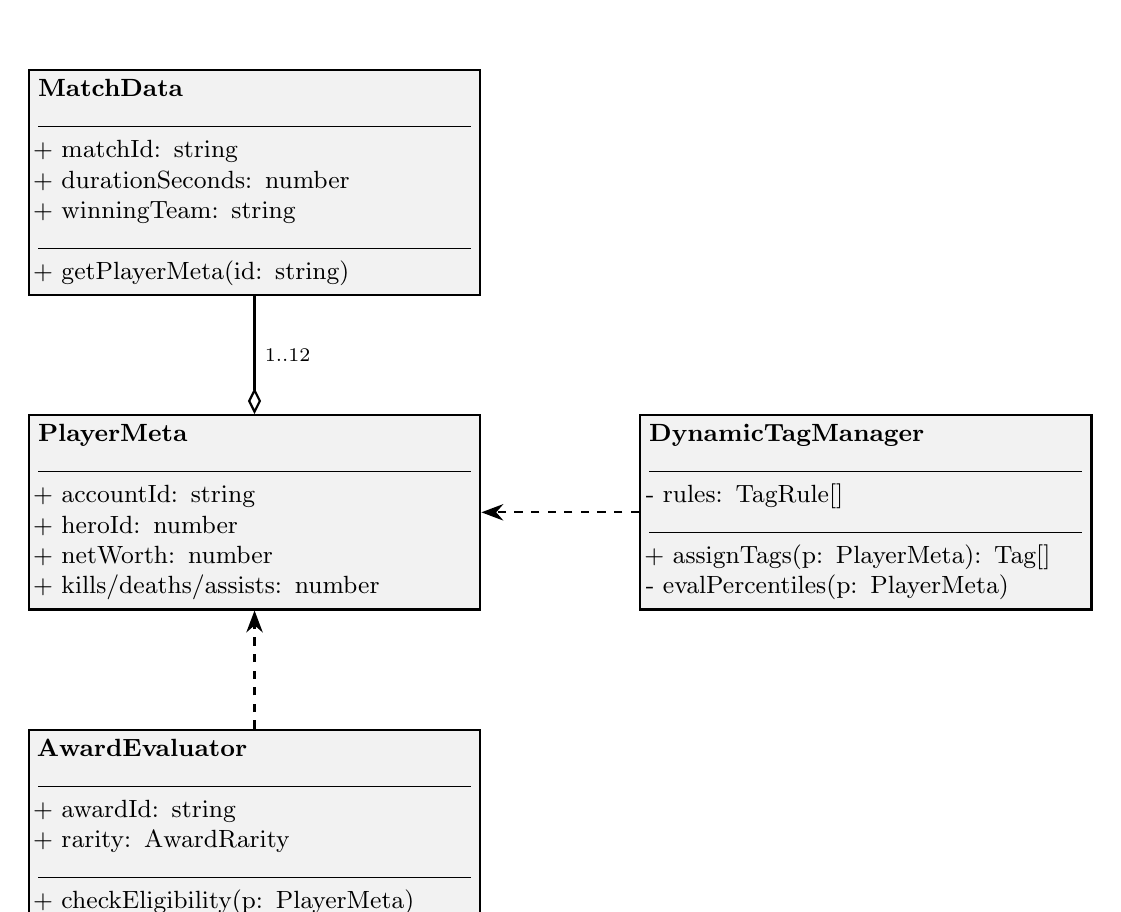
\begin{tikzpicture}[
    classbox/.style={rectangle, draw=black, thick, fill=gray!10, text width=5.5cm,
                     minimum height=1.5cm, align=left, font=\small},
    dependency/.style={-{Stealth[scale=1.2]}, dashed, thick},
    association/.style={-{Diamond[open, scale=1.2]}, thick}
]

\node[classbox] (Match) {
    \textbf{MatchData} \\
    \noindent\rule{\linewidth}{0.4pt}\\
    + matchId: string \\
    + durationSeconds: number \\
    + winningTeam: string \\
    \noindent\rule{\linewidth}{0.4pt}\\
    + getPlayerMeta(id: string)
};

\node[classbox] (Player) [below=1.5cm of Match] {
    \textbf{PlayerMeta} \\
    \noindent\rule{\linewidth}{0.4pt}\\
    + accountId: string \\
    + heroId: number \\
    + netWorth: number \\
    + kills/deaths/assists: number
};

\node[classbox] (TagManager) [right=2cm of Player] {
    \textbf{DynamicTagManager} \\
    \noindent\rule{\linewidth}{0.4pt}\\
    - rules: TagRule[] \\
    \noindent\rule{\linewidth}{0.4pt}\\
    + assignTags(p: PlayerMeta): Tag[] \\
    - evalPercentiles(p: PlayerMeta)
};

\node[classbox] (Award) [below=1.5cm of Player] {
    \textbf{AwardEvaluator} \\
    \noindent\rule{\linewidth}{0.4pt}\\
    + awardId: string \\
    + rarity: AwardRarity \\
    \noindent\rule{\linewidth}{0.4pt}\\
    + checkEligibility(p: PlayerMeta)
};

\draw[association] (Match) -- node[right, font=\scriptsize] {1..12} (Player);
\draw[dependency] (TagManager) -- (Player);
\draw[dependency] (Award) -- (Player);

\end{tikzpicture}
\caption{Diagramme de classes simplifié pour l'encapsulation et le traitement des entités du jeu.}
\label{fig:class_diagram}
\end{figure}

\subsection{Intégration OAuth --- Spotify}

L'authentification Spotify utilise le flux
\textit{Authorization Code with PKCE}. Un serveur HTTP local temporaire
sur le port 30765 réceptionne le callback OAuth. Pour résoudre l'injection
des clés API dans le build compilé, un système de credentials en fichier
JSON (placé dans le dossier \texttt{userData} d'Electron) a été mis en
place~:

\begin{lstlisting}[language=TypeScript,
  caption={Extrait de spotify-logic.ts --- chargement dynamique des identifiants}]
function loadCredentials() {
  // Chemin : ~/.config/DeadlockHelper/spotify-credentials.json (Linux)
  //       ou %APPDATA%\DeadlockHelper\spotify-credentials.json (Windows)
  const configPath = path.join(app.getPath('userData'),
                               'spotify-credentials.json');
  if (fs.existsSync(configPath)) {
    const raw = JSON.parse(fs.readFileSync(configPath, 'utf8'));
    return {
      clientId:     raw['clientId'],
      clientSecret: raw['clientSecret'],
      redirectUri:  raw['redirectUri'],
    };
  }
  // Repli sur les valeurs injectees au build (environnement de dev)
  return {
    clientId:     process.env.SPOTIFY_CLIENT_ID    ?? '',
    clientSecret: process.env.SPOTIFY_CLIENT_SECRET ?? '',
    redirectUri:  process.env.SPOTIFY_REDIRECT_URI
                  ?? 'http://127.0.0.1:30765/spotify/callback',
  };
}
\end{lstlisting}

\subsection{Python comme moteur de données et OCR}

Un processus Python~3.12 tourne en parallèle d'Electron. Il gère le
traitement des réponses JSON volumineuses de l'API et le worker OCR
(EasyOCR~+~thefuzz). Il communique avec Electron exclusivement via
\texttt{stdout} (JSON structuré) et \texttt{stderr} (diagnostics), sans
port réseau.

\begin{lstlisting}[language=Python,
  caption={Extrait de ocr-worker/main.py --- table des héros et sortie NDJSON}]
# Vocabulaire ferme des heros (hero_name -> hero_id officiel)
# Source : GET https://api.deadlock-api.com/v1/assets/heroes
HERO_MAP = {
    "Abrams": 6,  "Bebop": 15, "Billy": 63,  "Calico": 52,
    "Dynamo": 11, "Haze": 17,  "Infernus": 1, "Ivy": 20,
    "Kelvin": 12, "Lash": 16,  "McGinnis": 18,
    "Mo and Krill": 10, "Paradox": 22, "Pocket": 50,
    "Seven": 4,   "Shiv": 51,  "Warden": 27,  "Wraith": 8,
    # ... 28 heros au total
}

# Sortie NDJSON sur stdout (une ligne JSON par scan)
# Diagnostics sur stderr pour ne pas polluer le flux JSON
result = {"myTeam": my_team, "enemyTeam": enemy_team}
print(json.dumps(result), flush=True)   # lu par ipcMain d'Electron
\end{lstlisting}

\subsection{Récapitulatif des technologies}

\begin{center}
\begin{tabular}{ll}
\toprule
\textbf{Technologie} & \textbf{Rôle dans le projet} \\
\midrule
Electron 40.0.0 + Vite & Framework de bureau, bundler \\
TypeScript & Langage principal (main, renderer, preload) \\
Python 3.12 & Traitement de données, OCR \\
Tailwind CSS + ShadCN UI & Design system, composants UI \\
electron-store & Persistance locale (tokens, cache matchs, awards) \\
GitHub Actions & CI/CD --- compilation .AppImage et .exe \\
Deadlock-API.com & Données de matchs, héros, rang \\
Steam Web API (OpenID) & Authentification utilisateur \\
Spotify Web API (PKCE) & Contrôle de la lecture musicale \\
UptimeRobot & Monitoring heartbeat de l'API \\
EasyOCR + thefuzz & Reconnaissance de texte à l'écran (OCR) \\
\bottomrule
\end{tabular}
\end{center}

% ═══════════════════════════════════════════════════════════════════════════
\section{Nombre d'heures consacrées}
% ═══════════════════════════════════════════════════════════════════════════

Au départ du projet, une charge de travail de \textbf{150~heures} avait
été estimée pour l'ensemble du développement, de la planification à la
démonstration finale. En réalité, le projet a nécessité environ
\textbf{175~heures}, soit un dépassement de 25~heures. Ce surplus est
principalement attribuable à trois facteurs imprévus~: l'instabilité de
l'API communautaire (endpoints qui changent, données dépréciées à
filtrer), les problèmes de build CI/CD (CSP, injection des variables
d'environnement), et le temps investi dans l'exploration de solutions
alternatives pour le Live Dashboard et le worker OCR.

% ═══════════════════════════════════════════════════════════════════════════
\section{Ressources utilisées}
% ═══════════════════════════════════════════════════════════════════════════

\begin{description}[leftmargin=2cm, style=nextline]
  \item[\normalfont\textbf{Claude Code (Anthropic)}]
    Abonnement à 30\,\$/mois, utilisé durant le dernier mois de
    développement intensif pour l'assistance au code, la génération de
    documentation et la rédaction du présent rapport. Non prévu dans le
    budget initial~; dépense personnelle pour l'éducation.

  \item[\normalfont\textbf{Spotify Premium}]
    Abonnement à 12\,\$/mois pendant 5~mois (60\,\$ au total). Requis
    pour tester l'intégration du widget~: les fonctionnalités de contrôle
    de l'API Spotify nécessitent un compte Premium actif. Cette ressource
    était incluse dans le budget initial estimé.

  \item[\normalfont\textbf{Microsoft Planner}]
    Outil de gestion de projet (Kanban) inclus dans la suite Microsoft~365
    du Cégep. Aucun coût supplémentaire.

  \item[\normalfont\textbf{GitHub Actions}]
    CI/CD pour la compilation et la distribution automatisées. Gratuit
    dans le cadre du plan public GitHub.

  \item[\normalfont\textbf{Matériel}]
    Ordinateur personnel (dual-boot Windows~11 / CachyOS Linux) et
    un second écran pour tester l'application en conditions réelles de
    jeu (overlay in-game).
\end{description}

% ═══════════════════════════════════════════════════════════════════════════
\section{Sources d'information}
% ═══════════════════════════════════════════════════════════════════════════

\subsection{Fondations et environnement de développement}

\begin{itemize}
  \item \textbf{Electron.js}
    (\url{https://www.electronjs.org/}) --- Framework de référence pour
    créer des applications de bureau avec des technologies web. Point
    d'entrée principal de l'architecture.

  \item \textbf{Electron 40 --- Timeline}
    (\url{https://www.electronjs.org/fr/docs/latest/tutorial/electron-timelines})
    --- Consulté pour le choix de la version stable et la politique de
    support à long terme.

  \item \textbf{Python 3.12}
    (\url{https://docs.python.org/3.12/}) --- Référence officielle pour
    le moteur de données et le worker OCR.

  \item \textbf{Next.js}
    (\url{https://nextjs.org/docs}) --- Consulté pour les meilleures
    pratiques de routage et de performance, appliquées au renderer.

  \item \textbf{PEP 257}
    (\url{https://peps.python.org/pep-0257/}) --- Convention de
    documentation des docstrings Python, appliquée à \texttt{main.py}
    et \texttt{data\_processor.py}.
\end{itemize}

\subsection{APIs et données de jeu}

\begin{itemize}
  \item \textbf{Deadlock API}
    (\url{https://assets.deadlock-api.com/scalar} et
     \url{https://deadlock-api.com/}) --- Source principale de données~:
    historique des matchs, statistiques des héros, rang, scouting de
    joueurs.

  \item \textbf{UptimeRobot}
    (\url{https://dashboard.uptimerobot.com/monitors/802150090}) ---
    Monitoring de la disponibilité de l'API. Utilisé pour le heartbeat
    intégré à l'application (vérification toutes les 5~minutes).

  \item \textbf{Steam Web API}
    (\url{https://steamcommunity.com/dev}) --- Authentification OpenID
    et vérification de l'installation locale du jeu
    (\texttt{libraryfolders.vdf}).

  \item \textbf{Spotify Web API}
    (\url{https://developer.spotify.com/documentation/web-api}) ---
    Guide technique complet pour l'intégration du lecteur multimédia
    et le flux OAuth PKCE.
\end{itemize}

\subsection{Design, UX et inspiration}

\begin{itemize}
  \item \textbf{Tailwind CSS}
    (\url{https://tailwindcss.com/}) et \textbf{ShadCN UI}
    (\url{https://ui.shadcn.com/}) --- Design system utilisé pour
    construire une interface moderne, performante et cohérente.

  \item \textbf{Porofessor.gg}
    (\url{https://porofessor.gg/fr/}) et \textbf{U.gg}
    (\url{https://u.gg/}) --- Sites de référence du genre
    \textit{companion app} sur League of Legends, utilisés comme modèles
    pour l'organisation visuelle des statistiques et la création de
    tags clairs.
\end{itemize}

\subsection{Linux et overlay in-game}

\begin{itemize}
  \item \textbf{gtk-layer-shell}
    (\url{https://github.com/wmww/gtk-layer-shell}) --- Documentation
    sur les layers Wayland pour les fenêtres overlay.

  \item \textbf{MangoHud}
    (\url{https://github.com/flightlessmango/MangoHud}) --- Référence
    open-source d'overlay pour jeux Linux, consulté pour les bonnes
    pratiques de composition de fenêtres.
\end{itemize}

% ═══════════════════════════════════════════════════════════════════════════
\section{Difficultés rencontrées et solutions}
% ═══════════════════════════════════════════════════════════════════════════

\subsection{API communautaire instable et données dépréciées}

\textit{Deadlock-API.com} est une API communautaire non officielle, encore
en développement actif. Les noms d'endpoints changent, des héros retirés
du jeu restent dans les données, et certaines images pointent vers des URLs
invalides. La solution a été de maintenir une logique de filtrage côté
application~: ignorer les héros dont le champ \texttt{disabled} est
\texttt{true}, filtrer les images qui retournent une erreur 404, et mettre
en cache les données valides pour limiter les appels inutiles.

\subsection{Build CI/CD~: CSP et variables d'environnement}

Deux problèmes majeurs ont bloqué le pipeline GitHub Actions lors du
passage en production~:

\begin{enumerate}
  \item \textbf{Content Security Policy (CSP)~:} en mode production,
    Electron applique une CSP stricte qui bloquait l'affichage des images
    hébergées sur des domaines externes (pochettes Spotify sur
    \texttt{i.scdn.co}, avatars Steam, icônes de héros). La solution
    a été d'implémenter une double couche CSP~: une déclarée dans le
    processus principal via \texttt{session.defaultSession.webRequest\\
    .onHeadersReceived}, et une dans les entêtes HTML, en autorisant
    explicitement chaque domaine externe utilisé.

  \item \textbf{Variables d'environnement non injectées en production~:}
    les clés API définies dans \texttt{.env} ne suivent pas le build
    compilé. La solution a été de créer un fichier JSON de credentials
    placé dans le dossier \texttt{userData} d'Electron, accessible à
    l'exécution sans être embarqué dans le binaire distribué.
\end{enumerate}

\subsection{Live Dashboard~: limites du endpoint de parties actives}

Le premier plan pour le \textit{Live Dashboard} reposait sur l'endpoint
\texttt{/matches/active}. En pratique, il est limité aux 200~parties les
plus regardées (parties de haut rang ou en tournoi)~: les parties normales
n'y apparaissent jamais. De plus, le endpoint unitaire
\texttt{/v1/matches/\{id\}/metadata} est limité à 3~requêtes par heure et
dépend de Steam (retourne des erreurs 503 intermittentes).

La solution retenue a été de basculer vers le
\textit{bulk metadata endpoint}
(\texttt{GET /v1/matches/metadata?match\_ids=\{id\}}), qui offre un quota
de 10~requêtes par minute sans dépendance Steam. Un normaliseur a été
développé pour convertir son schéma vers le format attendu par l'interface
(les champs \texttt{team}, \texttt{game\_mode} et \texttt{winning\_team}
diffèrent entre les deux endpoints).

\subsection{OCR worker~: le défi du roster live}

Récupérer les noms et héros de chaque joueur \textit{pendant} une partie
s'est avéré être le défi technique le plus complexe. Trois approches ont
été tentées en séquence~:

\begin{enumerate}
  \item \textbf{Fichier \texttt{console.log} (-condebug)~:} le log de
    Deadlock ne contient que les informations du compte connecté et
    l'identifiant de la partie. Les noms et héros des autres joueurs
    n'y apparaissent pas.

  \item \textbf{Screenshot + OCR~:} un worker Python (EasyOCR~+~thefuzz)
    lit le panneau «~ESC~$>$~PLAYERS~» de Deadlock.
    \textbf{Résultat~: 12/12 héros identifiés (100\,\%)} et
    10/12 pseudos Steam. Limite fatale~: un pseudo Steam affiché
    en jeu n'est pas résolvable en \texttt{account\_id} (aucun endpoint
    Steam ou Deadlock ne supporte cette recherche), rendant les
    statistiques par joueur impossibles.

  \item \textbf{Attente post-partie~:} solution finale adoptée. Le
    Live Dashboard attend que la partie soit ingérée par l'API
    (quelques minutes après la fin), puis affiche les données complètes.
    Un mode MOCK dans les Paramètres permet de simuler un match en cours
    avec des données historiques.
\end{enumerate}

\subsection{Awards non calculables~: données absentes de l'API}

Sur les 48~awards définis, 21 ne peuvent pas être calculés~: les données
nécessaires sont absentes du payload \texttt{CMsgMatchMetaDataContents},
vérifié sur 153~clés distinctes d'une vraie réponse API. Les champs
manquants sont~: taux de tirs à la tête, compteurs de parries, dégâts
d'antiheal, dégâts par capacité individuelle et scores de catégories.
Ces 21~awards affichent «~Données indisponibles~» dans l'interface, avec
une explication explicite pour l'utilisateur.

% ═══════════════════════════════════════════════════════════════════════════
\section{Limites de la réalisation, et pourquoi}
% ═══════════════════════════════════════════════════════════════════════════

\begin{description}[leftmargin=2cm, style=nextline]
  \item[\normalfont\textbf{Roster en temps réel (Live Dashboard)}]
    L'API Deadlock n'expose les données d'une partie qu'après sa
    conclusion (ingestion post-partie). Il est donc impossible d'afficher
    les statistiques des joueurs \textit{pendant} une partie active. Un
    mode MOCK compense partiellement en permettant de simuler un match en
    cours avec des données historiques.

  \item[\normalfont\textbf{Overlay en mode fullscreen exclusif}]
    La propriété \texttt{alwaysOnTop} d'Electron ne passe pas au-dessus
    d'un jeu en mode fullscreen exclusif sous Linux/Wayland. L'overlay
    n'est visible que si le jeu tourne en mode \textit{Borderless
    Windowed}. Ce prérequis est documenté dans les Paramètres de
    l'application et vérifié au démarrage.

  \item[\normalfont\textbf{Composant Souls/min en overlay}]
    La quantité d'âmes ramassées par le joueur n'est disponible dans
    aucune source accessible en temps réel~: ni le \texttt{console.log},
    ni l'API active match, ni un GSI officiel de Valve. Le composant
    affiche «~\texttt{-- SPM}~» comme placeholder honnête.

  \item[\normalfont\textbf{OCR worker non intégré à Electron}]
    Le module Python EasyOCR fonctionne correctement en standalone
    (validé à 12/12 héros), mais son intégration dans Electron (spawn/kill
    du processus, lecture du flux NDJSON, toggle dans les Paramètres) n'a
    pas été finalisée. Même intégré, la limite de résolution des pseudos
    Steam en \texttt{account\_id} réduirait l'utilité du module aux seules
    données de héros.

  \item[\normalfont\textbf{21/48 awards indisponibles}]
    L'API ne fournit pas les données pour 21 des 48~awards. Cette limite
    est indépendante de l'application et dépend d'une éventuelle mise à
    jour de l'API communautaire ou d'une API officielle Valve.
\end{description}

% ═══════════════════════════════════════════════════════════════════════════
\section{Compétences du DEC réinvesties}
% ═══════════════════════════════════════════════════════════════════════════

Ce projet constitue l'aboutissement de ma formation et mobilise l'ensemble
des compétences acquises tout au long du DEC en Techniques de
l'informatique. Il ne s'agit pas uniquement d'écrire du code, mais
d'orchestrer plusieurs technologies pour répondre à un besoin utilisateur
concret, du même type que ceux rencontrés en milieu professionnel.

\textbf{Développement logiciel et web (420-VBA-LP, 420-V88-LP)~:}
l'interface construite avec Electron, Vite et TypeScript est une
application directe des cours de développement web~: gestion des
événements asynchrones, manipulation du DOM, routage entre pages, gestion
des états. L'utilisation de Tailwind CSS et ShadCN UI prolonge les bonnes
pratiques de mise en page apprises en cours.

\textbf{Programmation orientée objet (420-V83-LP)~:} la structure modulaire
du code repose sur des interfaces TypeScript strictement typées
(\texttt{AwardEntry}, \texttt{RichMatchMeta}, \texttt{GameState},
\texttt{OcrRoster}) qui encapsulent les données de chaque entité. Les
principes de séparation des responsabilités et d'encapsulation sont
appliqués systématiquement dans chaque module.

\textbf{Algorithmique et programmation avancée (420-V80-LP, 420-VA9-LP)~:}
le moteur Python traite des payloads JSON volumineux, calcule des métriques
par minute, et implémente une approximation des séquences de kills basée
sur l'analyse des intervalles temporels entre les morts.

\textbf{Systèmes d'exploitation (420-V89-LP)~:} l'adaptation
cross-platform (Windows~$\leftrightarrow$~Linux/Wayland) a exigé de
maîtriser la gestion des processus, les conventions de chemins, la
détection du répertoire Steam via \texttt{libraryfolders.vdf}, et les
contraintes de composition de fenêtres sous Wayland.

\textbf{Sécurité et automatisation (420-VB6-LP)~:} le pipeline CI/CD
GitHub Actions automatise la compilation et la distribution. La gestion
sécurisée des clés API (séparation build-time~vs.~runtime) et
l'implémentation de la CSP relèvent directement de ce domaine.

\textbf{Base de données (420-V91-LP)~:} \texttt{electron-store} joue le
rôle de base de données locale~: stockage des tokens, cache des
métadonnées de matchs, persistance des awards et TTL de 7~jours sur les
noms de joueurs.

\textbf{Mathématiques et statistiques (201-V03-LP, 201-V04-LP)~:} les
27~awards calculables reposent sur des métriques quantitatives (ratios,
seuils, percentiles) dérivées des statistiques de match.

\textbf{Gestion de projet (420-VB9-LP)~:} la planification Agile
(Kanban, MVP tagging, PRD) et la rigueur documentaire (ADR ---
\textit{Architecture Decision Records}) démontrent la capacité à mener
un projet complexe en solo sur plusieurs mois.

% ═══════════════════════════════════════════════════════════════════════════
\section{Analyse de conception : Cycle de vie et cheminement de pensée de l'onglet Live Dashboard}
% ═══════════════════════════════════════════════════════════════════════════

\subsection{Phase~1~: Identification des contraintes d'API et architecture de contournement}

La conception du \textit{Live Dashboard} a débuté par une hypothèse de travail intuitive~: interroger l'API individuellement pour chacun des 12~joueurs d'une partie, en récupérant leurs métadonnées de profil à la volée. Cette approche s'est révélée inapplicable dès la phase de prototypage. Le endpoint unitaire \texttt{GET /v1/matches/\{id\}/metadata} impose un \textit{rate limiting} sévère de \textbf{3~requêtes par heure}, rendant mécaniquement impossible l'interrogation successive de 12~joueurs dans une fenêtre de temps acceptable.

Face à cette contrainte structurelle, le raisonnement architectural a conduit à explorer les endpoints alternatifs disponibles dans la documentation de l'API. La solution identifiée est le \textit{bulk metadata endpoint}~: \texttt{GET /v1/matches/metadata?match\_ids=\{id\}}, conçu précisément pour centraliser en une seule requête l'ensemble des métadonnées d'une partie. Ce endpoint offre un quota de \textbf{10~requêtes par minute}, soit une amélioration d'un facteur~200 sur la fenêtre d'utilisation, et opère sans dépendance directe aux services Steam, éliminant les erreurs 503 intermittentes qui affectaient le endpoint unitaire. Ce choix illustre un principe fondamental de conception logicielle~: avant d'optimiser, il faut identifier et remettre en question les hypothèses de départ.

\subsection{Phase~2~: Design asynchrone et gestion d'état de l'interface}

La seconde difficulté architecturale concernait la réactivité de l'interface. Les requêtes réseau vers l'API Deadlock, dont les temps de réponse peuvent dépasser 800~ms, auraient gelé le fil d'exécution principal du renderer Chromium si elles avaient été exécutées de manière synchrone. Ce gel aurait produit une interface non réactive et une expérience utilisateur dégradée, particulièrement perceptible sur les animations de chargement.

La solution adoptée repose sur une \textbf{machine à états explicite} gouvernant le cycle de vie de l'onglet. Trois états distincts ont été définis et implémentés~:

\begin{enumerate}[leftmargin=*, label=\textbf{\arabic*.}]
  \item \textbf{Idle / Loading~:} état initial déclenché dès que l'utilisateur active l'onglet. L'interface affiche un \textit{shimmer effect} --- une animation CSS de squelette de contenu --- sur chaque tuile de joueur, signalant visuellement que les données sont en cours de récupération sans bloquer l'interaction.

  \item \textbf{Mutation / Parsing~:} état de traitement, activé à la réception de la réponse brute de l'API. Un normaliseur TypeScript transforme le schéma du \textit{bulk endpoint} (dont les champs \texttt{team}, \texttt{game\_mode} et \texttt{winning\_team} diffèrent du schéma unitaire) vers le type interne \texttt{RichMatchMeta}. Ce typage strict garantit que les composants d'interface ne reçoivent jamais de données partielles ou mal formées.

  \item \textbf{Final / Rendered~:} état terminal, déclenché après l'hydratation complète des données normalisées. Les tuiles de joueurs sont peuplées, les tags dynamiques sont appliqués via le \texttt{DynamicTagManager}, et les Awards de la partie sont calculés et affichés.
\end{enumerate}

Cette séparation claire des états élimine toute ambiguïté dans les transitions d'interface et facilite le débogage~: chaque état est observable et traçable indépendamment des autres.

\subsection{Phase~3~: Gestion défensive des cas d'erreur (Fallbacks)}

La troisième phase de conception a porté sur la résilience de l'onglet face aux défaillances de l'API. \textit{Deadlock-API.com}, en tant qu'API communautaire non officielle, est sujette à des interruptions de service, des erreurs 503 (\textit{Service Unavailable}) et des temps de réponse erratiques. Concevoir un \textit{Live Dashboard} qui refuse d'afficher quoi que ce soit en cas d'erreur aurait constitué une expérience utilisateur inacceptable.

La stratégie de \textbf{mode dégradé honnête} a été mise en place autour de la persistance locale via \texttt{electron-store}. Lors de chaque chargement réussi d'une partie, les métadonnées normalisées sont écrites en cache avec un \textbf{TTL de 7~jours}. En cas d'erreur 503 ou d'absence de connectivité lors d'une requête ultérieure, le système bascule automatiquement vers ces données en cache, avec un indicateur visuel clair informant l'utilisateur que les données affichées proviennent du dernier chargement réussi et peuvent ne pas être à jour.

Cette approche respecte deux principes fondamentaux~: la \textit{transparence} envers l'utilisateur, qui sait que les données sont issues du cache, et la \textit{continuité de service}, l'application restant fonctionnelle et utile même en cas de défaillance externe. Elle constitue une application directe des notions de persistance et de gestion de base de données étudiées dans le cadre du cours~420-V91-LP.

% ═══════════════════════════════════════════════════════════════════════════
\section{Bilan des apprentissages réalisés}
% ═══════════════════════════════════════════════════════════════════════════

\subsection{Apprentissages techniques}

\textbf{Architecture multi-processus Electron.}
Le concept le plus structurant du projet a été de comprendre et de
maîtriser l'architecture en trois couches d'Electron~: processus principal
(Node.js, accès système), preload script (pont de sécurité via
\texttt{contextBridge}), renderer (interface web Chromium). Chaque
message entre le renderer et le main doit passer par un canal IPC
explicitement déclaré~: cette rigueur m'a appris à concevoir des
interfaces logicielles compartimentées et sécurisées.

\textbf{Gestion d'une API instable et non officielle.}
Travailler avec une API communautaire en développement actif m'a appris
à anticiper les ruptures~: documenter chaque décision architecturale
(ADR), mettre en place des fallbacks, et concevoir des normaliseurs
robustes capables de gérer plusieurs versions d'un même schéma. C'est
une compétence directement transférable en milieu professionnel.

\textbf{Développement cross-platform Windows~$\leftrightarrow$~Linux.}
Porter l'application de Windows vers Linux/CachyOS/Wayland a mis en
lumière des différences profondes~: chemins de fichiers, gestion des
fenêtres (Wayland vs X11), permissions de processus. J'ai appris à
écrire du code conditionnel robuste et à tester sur les deux plateformes.

\textbf{Pipeline OAuth complet (PKCE).}
Implémenter le flux PKCE pour Spotify --- génération du
\textit{code verifier}, serveur HTTP local temporaire pour le callback,
gestion du refresh token, renouvellement automatique avant expiration ---
m'a donné une compréhension concrète des protocoles d'authentification
modernes.

\textbf{Python subprocess et communication NDJSON.}
Isoler le worker OCR (EasyOCR, PyTorch) dans un processus Python séparé,
communiquant avec Electron via \texttt{stdout} en JSON, m'a appris le
principe d'isolation des dépendances lourdes~: le renderer reste réactif
pendant que le worker traite des images en arrière-plan.

\textbf{Moteur d'awards --- logique algorithmique sur données réelles.}
Concevoir 48~métriques de performance et modéliser leurs seuils a nécessité
de raisonner rigoureusement sur les données disponibles~: quels champs
existent dans l'API, quelles approximations sont honnêtes, et comment
communiquer les limites à l'utilisateur.

\begin{lstlisting}[language=TypeScript,
  caption={Moteur des awards --- calcul par minute et approximation de killstreak}]
// Metrique de base : valeur divisee par la duree en minutes
function perMin(value: number, durationS: number): number {
  return durationS > 0 ? value / (durationS / 60) : 0;
}

// Approximation du killstreak : intervalles entre morts du joueur
function approxKillstreak(
  player: RichMetaPlayer,
  durationS: number,
): number | null {
  if (!player.death_details) return null;       // donnee absente
  if (player.death_details.length === 0) return player.kills;

  const snaps  = player.stats; // snapshots temporels cumulatifs
  const deaths = [...player.death_details]
    .sort((a, b) => a.game_time_s - b.game_time_s);

  // Construire les intervalles "sans mort"
  const intervals: Array<[number, number]> = [
    [0, deaths[0].game_time_s],
    ...deaths.slice(0, -1).map((d, i): [number, number] =>
      [d.game_time_s, deaths[i + 1].game_time_s]),
    [deaths[deaths.length - 1].game_time_s, durationS],
  ];

  let maxKills = 0;
  for (const [start, end] of intervals) {
    const w = (snapAtOrBefore(snaps, end)?.kills   ?? 0)
            - (snapAtOrBefore(snaps, start)?.kills ?? 0);
    if (w > maxKills) maxKills = w;
  }
  return maxKills; // approximation conservative (snapshots 3-6 min)
}
\end{lstlisting}

La logique de seuils des awards peut se représenter comme un arbre de
décision~:

\begin{figure}[htbp]
  \centering
  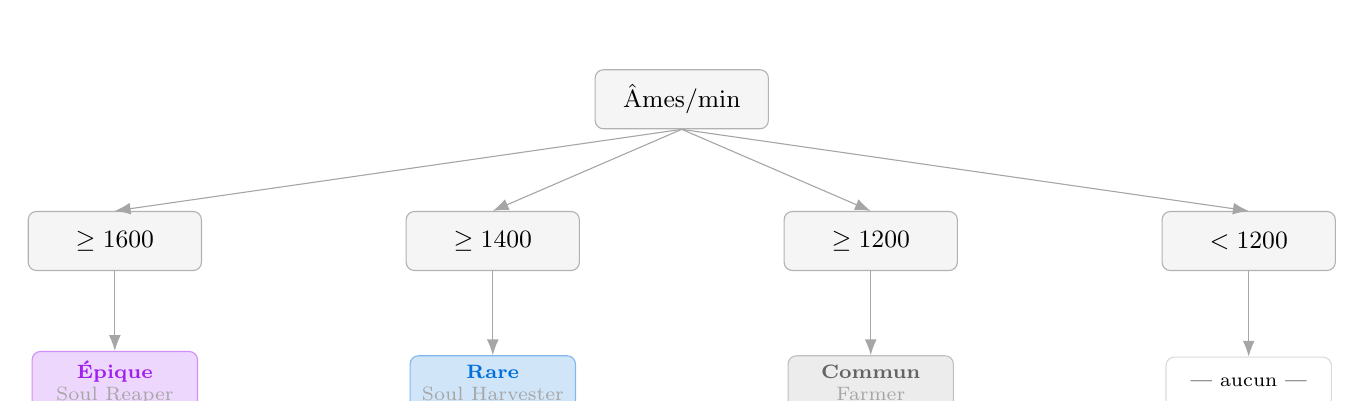
\begin{tikzpicture}[
    level distance=1.8cm,
    level 1/.style={sibling distance=4.8cm},
    level 2/.style={sibling distance=2.4cm},
    edge from parent/.style={draw, -{Latex[length=2mm]}, gray!70},
    every node/.style={font=\small},
    inner/.style={rectangle, draw=gray!60, rounded corners=3pt,
                  fill=gray!8, minimum width=2.2cm,
                  minimum height=0.75cm, align=center},
    leaf/.style={rectangle, rounded corners=3pt,
                 minimum width=2.1cm, minimum height=0.65cm, align=center,
                 font=\scriptsize},
  ]
    \node[inner] {Âmes/min}
      child { node[inner] {$\geq 1600$}
        child { node[leaf, fill=rarity-epic!18, draw=rarity-epic!50]
          {\textcolor{rarity-epic}{\textbf{Épique}}\\Soul Reaper} }
      }
      child { node[inner] {$\geq 1400$}
        child { node[leaf, fill=rarity-rare!18, draw=rarity-rare!50]
          {\textcolor{rarity-rare}{\textbf{Rare}}\\Soul Harvester} }
      }
      child { node[inner] {$\geq 1200$}
        child { node[leaf, fill=gray!15, draw=gray!50]
          {\textcolor{rarity-common}{\textbf{Commun}}\\Farmer} }
      }
      child { node[inner] {$< 1200$}
        child { node[leaf, fill=white, draw=gray!30]
          {--- aucun ---} }
      };
  \end{tikzpicture}
  \caption{Arbre de décision des awards basés sur les âmes par minute}
  \label{fig:awards-tree}
\end{figure}

La figure~\ref{fig:awards-tree} illustre le cas archétypal des awards~: une seule métrique scalaire comparée à des seuils hiérarchisés. Deux autres familles méritent une analyse approfondie, car leur évaluation implique une logique de calcul sensiblement plus complexe. Dans les deux cas, les données brutes arrivent sous forme de l'objet \texttt{RichMatchMeta}~: la réponse JSON de l'endpoint \texttt{GET /v1/matches/metadata?match\_ids=\{id\}} est transmise du processus principal au renderer via le canal IPC (\texttt{ipcRenderer.invoke('api:request', ...)}\,), puis désérialisée et passée directement à \texttt{computeAwardsForMatch}.

\medskip\textbf{Famille Kill Participation --- double condition simultanée.}

Les awards de participation aux éliminations imposent une \textbf{double condition conjonctive}~: le joueur doit simultanément dépasser un seuil absolu d'actions (20 kills~+~assists cumulés) \textit{et} un pourcentage du total de kills de son équipe. La figure~\ref{fig:awards-kp} illustre cet arbre à deux niveaux de décision.

\begin{figure}[htbp]
\centering
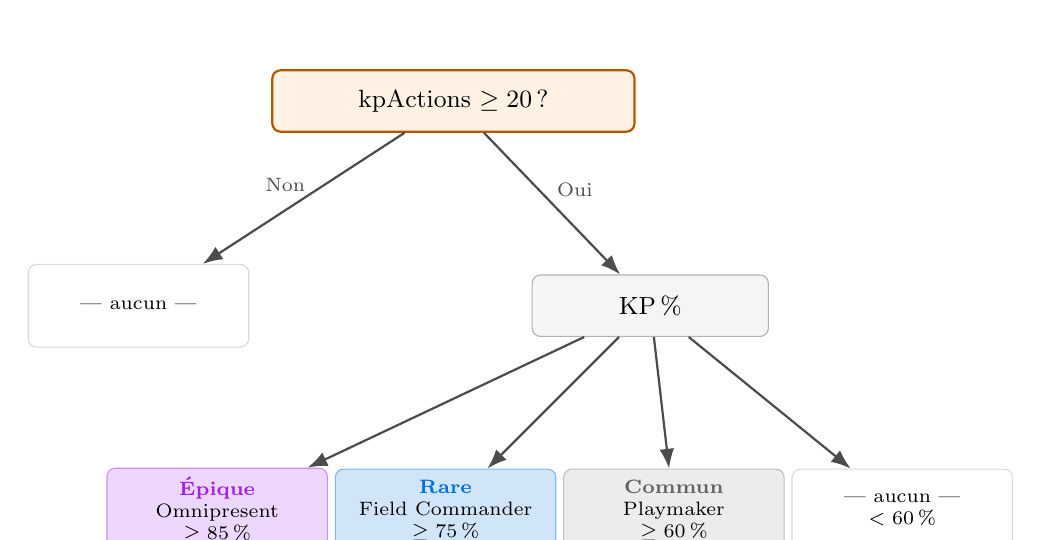
\begin{tikzpicture}[
    inner/.style={rectangle, draw=gray!60, rounded corners=3pt,
                  fill=gray!8, minimum width=3cm,
                  minimum height=0.78cm, align=center, font=\small},
    gate/.style={rectangle, draw=orange!70!black, rounded corners=3pt,
                 fill=orange!10, minimum width=4.6cm,
                 minimum height=0.78cm, align=center, font=\small, thick},
    leaf/.style={rectangle, rounded corners=3pt,
                 minimum width=2.8cm, minimum height=1.05cm,
                 align=center, font=\scriptsize},
    arr/.style={-{Latex[length=2.5mm]}, thick, gray!60!black},
]

\node[gate] (gate) at (4, 0) {kpActions $\geq 20$\,?};

\node[leaf, fill=white, draw=gray!30] (none0) at (0, -2.6)
    {--- aucun ---};

\node[inner] (kp) at (6.5, -2.6) {KP\,\%};

\node[leaf, fill=rarity-epic!18, draw=rarity-epic!50] (epic) at (1, -5.2)
    {\textcolor{rarity-epic}{\textbf{Épique}}\\
     Omnipresent\\$\geq 85\,\%$};

\node[leaf, fill=rarity-rare!18, draw=rarity-rare!50] (rare) at (3.9, -5.2)
    {\textcolor{rarity-rare}{\textbf{Rare}}\\
     Field Commander\\$\geq 75\,\%$};

\node[leaf, fill=gray!15, draw=gray!50] (comm) at (6.8, -5.2)
    {\textcolor{rarity-common}{\textbf{Commun}}\\
     Playmaker\\$\geq 60\,\%$};

\node[leaf, fill=white, draw=gray!30] (none1) at (9.7, -5.2)
    {--- aucun ---\\$< 60\,\%$};

\draw[arr] (gate) -- node[left=3pt, font=\scriptsize, pos=0.4] {Non} (none0);
\draw[arr] (gate) -- node[right=3pt, font=\scriptsize, pos=0.4] {Oui} (kp);
\draw[arr] (kp) -- (epic);
\draw[arr] (kp) -- (rare);
\draw[arr] (kp) -- (comm);
\draw[arr] (kp) -- (none1);

\end{tikzpicture}
\caption{Arbre de décision des awards Kill Participation~--- porte d'entrée absolue (kpActions) et seuils de pourcentage hiérarchisés.}
\label{fig:awards-kp}
\end{figure}

Un comportement important de cette famille est la \textbf{cumulabilité des awards}~: les trois conditions sont des blocs \texttt{if} séquentiels indépendants, et non une structure \texttt{else if}. Un joueur atteignant $85\,\%$ de KP avec 25~actions décroche simultanément \textit{Omnipresent}, \textit{Field Commander} et \textit{Playmaker}. Le champ \texttt{teamKills} n'est pas fourni directement par l'API~; il est recalculé dans le renderer en filtrant \texttt{meta.players} sur \texttt{p.team === player.team} et en sommant les kills~: un calcul local qui garantit la cohérence avec le payload reçu sans requête réseau supplémentaire.

\medskip\textbf{Famille Killstreak --- approximation par intervalles inter-morts.}

Les awards de killstreak (\textit{On Fire}~10, \textit{Heat Wave}~15, \textit{Blaze of Glory}~20) sont les plus algorithmiquement complexes du moteur. L'API Deadlock ne fournit aucun horodatage individuel par élimination~: la série maximale doit être \textbf{approximée} à partir de deux structures présentes dans \texttt{RichMatchMeta}. La figure~\ref{fig:awards-killstreak} illustre le flux de calcul complet, de la réception des données à l'attribution des awards.

\begin{figure}[htbp]
\centering
\begin{tikzpicture}[
    step/.style={rectangle, draw=gray!60, rounded corners=4pt,
                 fill=gray!8, minimum width=8.2cm, minimum height=0.82cm,
                 align=center, font=\small},
    data/.style={rectangle, draw=blue!50!black, rounded corners=4pt,
                 fill=blue!8, minimum width=8.2cm, minimum height=0.82cm,
                 align=center, font=\small, dashed, thick},
    leaf/.style={rectangle, rounded corners=3pt,
                 minimum width=2.8cm, minimum height=1.05cm,
                 align=center, font=\scriptsize},
    arr/.style={-{Latex[length=2.5mm]}, thick, gray!60!black},
]

\node[data] (api) at (4.1, 0)
    {\textsc{ipc} $\to$ \texttt{death\_details[]\{game\_time\_s\}} $+$ \texttt{stats[]\{time\_stamp\_s,\ kills\}}};

\node[step] (srt) at (4.1, -1.6)
    {1.~Trier \texttt{death\_details} par \texttt{game\_time\_s} croissant};

\node[step] (ivl) at (4.1, -3.2)
    {2.~Construire les intervalles~:\ $[\,0,\,d_1\,],\ [\,d_1,\,d_2\,],\ \ldots,\ [\,d_n,\,T\,]$};

\node[step] (dlt) at (4.1, -4.8)
    {3.~$\Delta\text{kills}_i\ =\ \text{kills}(t_{\text{fin},i})\ -\ \text{kills}(t_{\text{début},i})$
     \quad via snapshots \texttt{stats[]}};

\node[step] (mxk) at (4.1, -6.4)
    {4.~$\text{maxKills}\ =\ \max_i\!\left(\Delta\text{kills}_i\right)$
     \ $\leftarrow$ série approximée \textit{(biais conservateur)}};

\node[leaf, fill=rarity-uncommon!18, draw=rarity-uncommon!60] (onfire) at (1.2, -8.6)
    {\textcolor{rarity-uncommon}{\textbf{Uncommon}}\\On Fire\\$\geq 10$};

\node[leaf, fill=rarity-rare!18, draw=rarity-rare!50] (heat) at (4.1, -8.6)
    {\textcolor{rarity-rare}{\textbf{Rare}}\\Heat Wave\\$\geq 15$};

\node[leaf, fill=rarity-epic!18, draw=rarity-epic!50] (blaze) at (7.0, -8.6)
    {\textcolor{rarity-epic}{\textbf{Épique}}\\Blaze of Glory\\$\geq 20$};

\draw[arr] (api) -- (srt);
\draw[arr] (srt) -- (ivl);
\draw[arr] (ivl) -- (dlt);
\draw[arr] (dlt) -- (mxk);
\draw[arr] (mxk) -- (onfire);
\draw[arr] (mxk) -- (heat);
\draw[arr] (mxk) -- (blaze);

\end{tikzpicture}
\caption{Diagramme de flux de l'approximation du killstreak~--- intervalles inter-morts et snapshots cumulatifs \texttt{stats[]}, reçus via IPC.}
\label{fig:awards-killstreak}
\end{figure}

L'approximation présente un \textbf{biais conservateur intentionnel}~: les snapshots \texttt{stats[]} sont capturés toutes les 3~à~6~minutes, et non à chaque kill. Si un joueur enchaîne 8~kills dans un intervalle de 90~secondes entre deux morts rapprochées, mais que le snapshot le plus proche date d'avant cet intervalle, seuls les kills visibles dans la plage temporelle du snapshot seront comptés. L'award n'est accordé que si le seuil est atteint malgré cette sous-estimation~: c'est une décision délibérée qui garantit qu'aucun award de killstreak n'est décerné à tort.

Deux cas limites critiques sont gérés explicitement~: (1)~si \texttt{death\_details} est absent du payload (certains matchs archivés n'exposent pas ce champ), la fonction retourne \texttt{null} et les trois awards sont entièrement ignorés pour ce match plutôt que d'afficher une valeur erronée~; (2)~si \texttt{death\_details.length === 0} (partie parfaite sans aucune mort), l'intégralité de \texttt{player.kills} constitue une seule séquence ininterrompue et est retournée directement, sans construction d'intervalles. Ces deux garde-fous illustrent le même principe de programmation défensive que \texttt{Math.max(1, stats.deaths)} dans \texttt{DynamicTagManager}~: préférer un résultat absent à un résultat incorrect.

\bigskip

Le module \texttt{DynamicTagManager}, présenté ci-après, illustre un second réinvestissement de ces mêmes compétences, appliqué cette fois à la classification comportementale des joueurs en temps réel.

\begin{lstlisting}[language=TypeScript,
  caption={DynamicTagManager --- classification comportementale par métriques de performance}]
// src/services/TagManager.ts
export interface PlayerPerformance {
    kills: number;
    deaths: number;
    assists: number;
    netWorth: number;
    damageMitigated: number;
    objectiveDamage: number;
    gameDurationMin: number;
}

export type PlaystyleTag =
    | 'GLASS_CANNON'
    | 'OBJECTIVE_BEAST'
    | 'TACTICAL_FEEDER'
    | 'GOLD_MINER';

export class DynamicTagManager {
    public static generateTags(
        stats: PlayerPerformance,
    ): PlaystyleTag[] {
        const tags: PlaystyleTag[] = [];

        // Math.max(1, deaths) : programmation defensive contre la division
        // par zero lors d'une partie parfaite (0 mort)
        const kda =
            (stats.kills + stats.assists) /
            Math.max(1, stats.deaths);
        const gpm = stats.netWorth / stats.gameDurationMin;
        const objPerMin =
            stats.objectiveDamage / stats.gameDurationMin;

        if (kda > 3.5 && stats.deaths > stats.kills * 1.2) {
            tags.push('GLASS_CANNON');
        }
        if (objPerMin > 150) {
            tags.push('OBJECTIVE_BEAST');
        }
        if (gpm > 1100) {
            tags.push('GOLD_MINER');
        }
        if (kda < 1.0 && (stats.kills + stats.assists) > 15) {
            tags.push('TACTICAL_FEEDER');
        }

        return tags;
    }
}
\end{lstlisting}

Ce module démontre le réinvestissement concret des notions d'algorithmique et de statistiques quantitatives du DEC. Les métriques calculées --- KDA, GPM et dégâts d'objectif par minute --- sont des ratios normalisés qui permettent de comparer des joueurs indépendamment de la durée de la partie, un raisonnement directement issu des cours de mathématiques appliquées (201-V03-LP) et d'algèbre et statistiques (201-V04-LP).

Un aspect particulièrement représentatif de la \textbf{programmation défensive} est l'expression \texttt{Math.max(1, stats.deaths)} au calcul du KDA. Sans cette protection, une partie parfaite --- où un joueur terminerait avec \textbf{zéro mort} --- provoquerait une division par zéro, produisant un résultat \texttt{Infinity} ou \texttt{NaN} en JavaScript. Ces valeurs se propagent silencieusement dans les calculs suivants, corrompent les comparaisons conditionnelles (\texttt{Infinity > 3.5} évalue à \texttt{true}, ce qui déclencherait faussement le tag \texttt{GLASS\_CANNON}), et peuvent ultimement faire crasher un composant d'interface en arrière-plan. Le \texttt{Math.max(1,~stats.deaths)} ramène le dénominateur à~1 au minimum, garantissant que le résultat reste un nombre fini et sémantiquement cohérent quel que soit le scénario de jeu, y compris les cas limites statistiquement rares mais tout à fait légitimes.

\textbf{Rédaction d'un rapport professionnel en \LaTeX{}.}
La production de ce document officiel m'a initié à la typographie
professionnelle avec \LaTeX{}~: maîtrise des environnements
(\texttt{lstlisting} pour le code, \texttt{tikzpicture} pour les
diagrammes, \texttt{figure} pour les captures d'écran, \texttt{tabular}
pour les tableaux), gestion des flottants, configuration de Babel pour
le français, et génération automatique de la table des matières et de la
liste des figures. Cette rigueur de mise en page est directement applicable
à la rédaction de documentation technique professionnelle.

\subsection{Apprentissages en gestion de projet et outils}

\textbf{Obsidian et Microsoft Planner comme colonne vertébrale.}
L'utilisation combinée d'Obsidian (notes structurées, diagrammes
Excalidraw, liens bidirectionnels entre concepts) et de Microsoft Planner
(Kanban, tags MVP~vs.~Backlog) m'a appris à \textit{externaliser} la
complexité~: plutôt que de garder les décisions en tête, je les
matérialise dans des outils dédiés. Cette habitude réduit la charge
cognitive, améliore la qualité des décisions et produit une traçabilité
naturelle de l'évolution du projet.

\textbf{Claude Code, skills et MCP servers --- orchestrer l'IA comme outil
professionnel.}
Ce projet m'a permis de développer une compétence émergente~: savoir
«~orchestrer~» un assistant IA de développement. Au-delà de la génération
de code, j'ai appris à utiliser des \textit{skills} spécialisés~:
\texttt{/grill-me} pour valider un plan technique face à des questions
précises, \texttt{/grill-with-docs} pour confronter une décision à la
documentation et aux ADR existants, et \texttt{/latex-handouts} pour
produire ce rapport officiel. Les \textit{MCP servers}
(\textit{Model Context Protocol}) m'ont appris à donner à l'IA un accès
structuré au projet~: fichiers, historique Git, documentation, afin d'obtenir
des réponses contextualisées plutôt que génériques. Apprendre à formuler
le bon contexte, à valider les réponses et à itérer rapidement est une
compétence professionnelle que ce projet m'a permis de développer
concrètement.

% =============================================================================
\end{document}
